% ============================================================
%  tikz_fig_did.tex
%  Difference-in-Differences（DiD）の概念図
%
%  【単体コンパイル】
%    uplatex  tikz_fig_did.tex && dvipdfmx tikz_fig_did.dvi
%
%  【Beamer への組み込み】
%    \input{tikz/tikz_fig_did}
%
%  設定値:
%    Y_{C,0}   = 2.0  （対照群・処置前）
%    Y_{T,0}   = 4.5  （処置群・処置前）
%    Y_{C,1}   = 3.5  （対照群・処置後）
%    Y_{T,1}   = 7.5  （処置群・処置後・実績）
%    Y_{CF,1}  = 6.0  （処置群・処置後・反事実）
%                     = Y_{T,0} + (Y_{C,1} - Y_{C,0}) = 4.5 + 1.5
%
%    DiD = (Y_{T,1} - Y_{T,0}) - (Y_{C,1} - Y_{C,0})
%        = (7.5 - 4.5)         - (3.5 - 2.0)
%        = 3.0                 - 1.5          = 1.5
%
%  コメントアウトで以下も用意:
%    (A) 変化分解の縦矢印（ΔY_T, ΔY_C を右端に並置）
%    (B) DiD 公式テキスト
% ============================================================
\documentclass[tikz, dvipdfmx]{standalone}
\usepackage{tikz}
\usetikzlibrary{arrows.meta, decorations.pathreplacing}
\definecolor{gdpblue} {RGB}{30,  90,  180}
\definecolor{trendred}{RGB}{190, 40,  40}
\definecolor{cfgray}  {RGB}{100, 140, 200}   % 反事実（薄い青）

\begin{document}
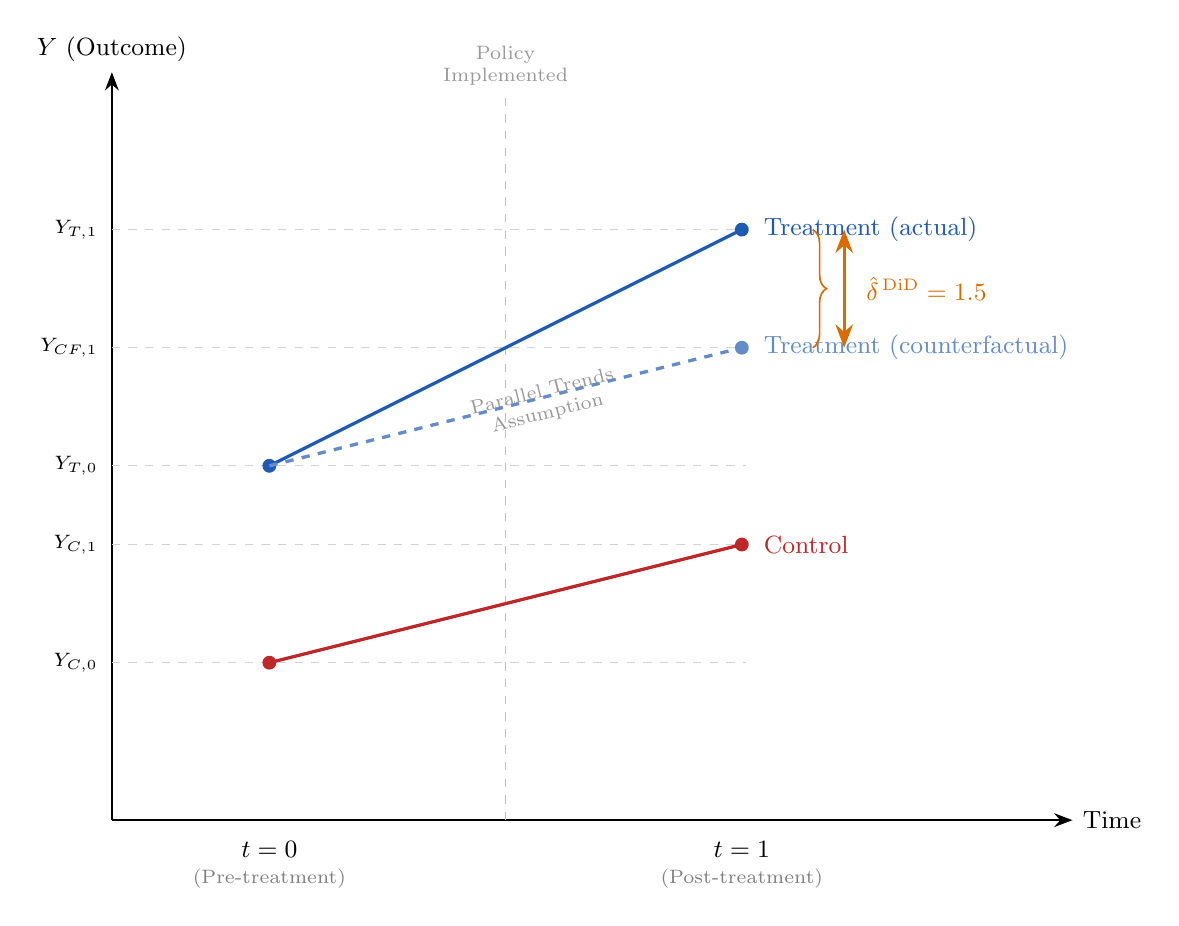
\begin{tikzpicture}[
  >=Stealth,
  thick,
]

%% ─── 座標系 ────────────────────────────────────────────────
%%  横軸: x ∈ [0, 12]
%%  Pre 点  x = 2,  Post 点 x = 8,  Policy 縦線 x = 5
%%  縦軸: y ∈ [0, 9]

% ── 軸 ──────────────────────────────────────────────────────
\draw[->] (0,0) -- (12.2,0)
  node[right, font=\small] {Time};
\draw[->] (0,0) -- (0,9.5)
  node[above, font=\small] {$Y$ (Outcome)};

% ── Pre / Post ラベル ────────────────────────────────────────
\node[below=4pt, font=\small] at (2,0) {$t=0$};
\node[below=14pt, font=\scriptsize, gray] at (2,0) {(Pre-treatment)};
\node[below=4pt, font=\small] at (8,0) {$t=1$};
\node[below=14pt, font=\scriptsize, gray] at (8,0) {(Post-treatment)};

% ── Policy Implementation 縦破線 ────────────────────────────
\draw[gray!50, thin, dashed] (5,0) -- (5,9.2);
\node[above, font=\scriptsize, gray!80, align=center] at (5,9.2)
  {Policy\\Implemented};

% ── 縦軸の参照点（水平点線 + ラベル） ───────────────────────
% Y_{C,0} = 2.0
\draw[gray!35, thin, dashed] (0,2.0) -- (8.05,2.0);
\node[left, font=\scriptsize] at (-0.05,2.0) {$Y_{C,0}$};

% Y_{C,1} = 3.5
\draw[gray!35, thin, dashed] (0,3.5) -- (8.05,3.5);
\node[left, font=\scriptsize] at (-0.05,3.5) {$Y_{C,1}$};

% Y_{T,0} = 4.5
\draw[gray!35, thin, dashed] (0,4.5) -- (8.05,4.5);
\node[left, font=\scriptsize] at (-0.05,4.5) {$Y_{T,0}$};

% Y_{CF,1} = 6.0
\draw[gray!35, thin, dashed] (0,6.0) -- (8.05,6.0);
\node[left, font=\scriptsize] at (-0.05,6.0) {$Y_{CF,1}$};

% Y_{T,1} = 7.5
\draw[gray!35, thin, dashed] (0,7.5) -- (8.05,7.5);
\node[left, font=\scriptsize] at (-0.05,7.5) {$Y_{T,1}$};


% ════════════════════════════════════════════════════════════
%  主要曲線
% ════════════════════════════════════════════════════════════

% ── 対照群 Control（赤実線） ─────────────────────────────────
\draw[trendred, very thick] (2,2.0) -- (8,3.5);
\fill[trendred] (2,2.0) circle[radius=2.5pt];
\fill[trendred] (8,3.5) circle[radius=2.5pt];
\node[right, font=\small, trendred] at (8.15,3.5)
  {Control};

% ── 処置群 実績 Treatment actual（青実線） ───────────────────
\draw[gdpblue, very thick] (2,4.5) -- (8,7.5);
\fill[gdpblue] (2,4.5) circle[radius=2.5pt];
\fill[gdpblue] (8,7.5) circle[radius=2.5pt];
\node[right, font=\small, gdpblue] at (8.15,7.5)
  {Treatment (actual)};

% ── 反事実 Counterfactual（青系の破線）──────────────────────
%    傾き = 対照群と同じ = (3.5-2.0)/(8-2) = 0.25/unit
%    Y_{CF}(x) = 4.5 + 0.25*(x-2)
%    x=8 → Y_{CF,1} = 4.5 + 1.5 = 6.0 ✓
\draw[cfgray, very thick, dashed] (2,4.5) -- (8,6.0);
\fill[cfgray] (8,6.0) circle[radius=2.5pt];
\node[right, font=\small, cfgray] at (8.15,6.0)
  {Treatment (counterfactual)};


% ════════════════════════════════════════════════════════════
%  DiD 推定量のアノテーション
% ════════════════════════════════════════════════════════════

% ── DiD 縦の両矢印（Y_{CF,1} ↔ Y_{T,1}） ────────────────────
\draw[<->, very thick, orange!85!black]
  (9.3, 6.0) -- (9.3, 7.5);
\node[right, font=\small, orange!85!black, align=left]
  at (9.45, 6.75)
  {$\hat{\delta}^{\,\mathrm{DiD}} = 1.5$};

% ── 波括弧で DiD の範囲を強調 ─────────────────────────────
\draw[decorate,
  decoration={brace, amplitude=5pt, mirror},
  orange!85!black, semithick]
  (8.9, 6.0) -- (8.9, 7.5);

% ── Parallel Trends 注釈 ────────────────────────────────────
%    対照群と反事実の傾きが等しいことを示す
%    傾き = arctan(0.25) ≈ 14°
\node[font=\scriptsize, gray!80, rotate=14, align=center]
  at (5.5, 5.3)
  {Parallel Trends\\Assumption};


% ════════════════════════════════════════════════════════════
%  コメントアウト: 変化分解の縦矢印（右端に並置）
% ════════════════════════════════════════════════════════════

%% ── (A) ΔY_T（処置群の変化）: x=10.8 ──────────────────────
%% \draw[<->, semithick, gdpblue!80]
%%   (10.8, 4.5) -- (10.8, 7.5);
%% \draw[dashed, gray!30, thin] (0,4.5) -- (10.8,4.5);
%% \draw[dashed, gray!30, thin] (0,7.5) -- (10.8,7.5);
%% \node[right, font=\scriptsize, gdpblue!80] at (10.9, 6.0)
%%   {$\Delta Y_T = 3.0$};
%%
%% ── (B) ΔY_C（対照群の変化）: x=11.5 ──────────────────────
%% \draw[<->, semithick, trendred!80]
%%   (11.5, 2.0) -- (11.5, 3.5);
%% \node[right, font=\scriptsize, trendred!80] at (11.6, 2.75)
%%   {$\Delta Y_C = 1.5$};
%%
%% ── (C) DiD 公式テキスト ─────────────────────────────────
%% \node[align=left, font=\scriptsize, gray!80] at (9.5, 1.2) {%
%%   $\hat{\delta}^{\,\mathrm{DiD}}$
%%   $= \underbrace{(Y_{T,1}-Y_{T,0})}_{3.0}
%%      - \underbrace{(Y_{C,1}-Y_{C,0})}_{1.5} = 1.5$};

\end{tikzpicture}
\end{document}
